\documentclass[letterpaper,12pt,notitlepage,twoside]{report}

\newcommand{\watermark}{MLOps}
\newcommand{\booktopic}{Machine Learning Operations}
\newcommand{\lastname}{Okoli}
\usepackage{NoteStyle}
\usepackage{placeins}
\usepackage{listings}
\usepackage{pifont}

\definecolor{firebrick}{rgb}{0.7, 0.13, 0.13}

\definecolor{codegreen}{rgb}{0,0.6,0}
\definecolor{codegray}{rgb}{0.5,0.5,0.5}
\definecolor{codepurple}{rgb}{0.58,0,0.82}
\definecolor{backcolour}{rgb}{0.95,0.95,0.92}

\lstdefinestyle{mystyle}{
    backgroundcolor=\color{backcolour},   
    commentstyle=\color{codegreen},
    keywordstyle=\color{magenta},
    numberstyle=\tiny\color{codegray},
    stringstyle=\color{codepurple},
    basicstyle=\ttfamily\footnotesize,
    breakatwhitespace=false,         
    breaklines=true,                 
    captionpos=b,                    
    keepspaces=true,                 
    numbers=left,                    
    numbersep=5pt,                  
    showspaces=false,                
    showstringspaces=false,
    showtabs=false,                  
    tabsize=2
}

% Prevents hypenation 
\tolerance=1
\emergencystretch=\maxdimen
\hbadness=10000


\lstset{style=mystyle}

\title{Machine Learning Operations}
\author{Chuks Okoli}
\date{\footnotesize Last Updated: \today}

\hypersetup{
  pdftitle={Machine Learning Operations},
  pdfauthor={Chuks Okoli},
  pdfsubject={},
}

% ToC on the title page:
% https://tex.stackexchange.com/a/45863
\makeatletter
\newcommand*{\toccontents}{\@starttoc{toc}}
\makeatother

\begin{document}

\begin{titlepage}
  \pagestyle{plain}
  \maketitle
  \setcounter{tocdepth}{2}

  \pdfbookmark[section]{\contentsname}{toc}
  \toccontents
  % Separate page:
  % \tableofcontents
\end{titlepage}

%------------------- Chapter 1: Introduction  -----------------%
\chapter{Introduction} \label{ch:1}

\firstletter{Hello there}, and welcome to \booktopic. This work is a culmination of hours of effort to create my reference for machine learning operations. All of the explanations are in my own words but majority of the content are based on Alexey Grigorev's DataTalksClub \href{https://github.com/DataTalksClub/mlops-zoomcamp}{MLOps Zoomcamp course}.

\begin{mathaside}[frametitle=\mathtitle{Explaining MLOps to a \color{firebrick}{5 year old}}]
\textit{Imagine you have a magical garden. In this garden, you have a special plant that can grow different kinds of fruits, but you need to take good care of it.}

\textit{MLOps is like having a magical gardener to help you. This gardener does three important things:}
\begin{enumerate}
    \item \textit{\textbf{Teaching the Plant}: The gardener shows the plant pictures of different fruits (like apples, oranges, and bananas) so it can learn to grow them. This is like the gardener helping the plant understand what to do. In MLOps, this is called training a machine learning model.}
    
    \item \textit{\textbf{Taking Care of the Garden}: The gardener makes sure the soil is rich, the water is just right, and there are no weeds. The gardener also provides the plant with the best tools and instructions to grow healthy fruits. In MLOps, this is called managing the infrastructure for the machine learning model.}
    
    \item \textit{\textbf{Sharing the Fruits}: Once the plant grows the fruits, the gardener picks them and puts them in baskets for everyone to enjoy. The gardener makes sure the fruits are easy to find and delicious. In MLOps, this is called deploying the model so it can be used for something useful.}
\end{enumerate}

\textit{Here's the magical part: The gardener watches over the garden to make sure everything is running smoothly. If a bug tries to eat the plant or if the plant stops growing fruits, the gardener fixes the problem right away.}

\textit{So, MLOps is like having a magical gardener who helps your special plant (machine learning model) stay happy, healthy, and productive, making sure it grows the best fruits for everyone to enjoy!}
\end{mathaside}


\section{What is MLOps?}
\inspiration{MLOps, also known as DevOps for machine learning, is an umbrella term that encompasses philosophies, practices, and technologies that are related to implementing machine learning lifecycles in a production environment.}{Microsoft Blog}{}

Machine Learning Operations (MLOps) is a set of best practices for putting machine learning models into production. The process for a machine learning project involves:
\begin{itemize}
	\item Design - define if machine learning is the right tool for solving the problem
	\item Train - train the model to find the best possible model
	\item Operate - deploy the model,  and monitor degradation or quality of the model
\end{itemize}
MLOps is a set of practices for automating everything and working together as a team on a machine learning project.

 \begin{funfact}[frametitle=\facttitlep{Fun Fact}{MLOps Principles}]
As machine learning and AI become more common in software, it's important to create guidelines and tools for testing, deploying, managing, and monitoring ML models in real-world use. This is where MLOps comes in. It helps prevent ``technical debt'' in machine learning projects by ensuring smooth operation and maintenance of models throughout their lifecycle.
\end{funfact}

MLOps helps to manage and orchestrate the end-to-end machine learning lifecycle by ensuring models are consistently accessible, reproducible, and scalable. It focuses on automating deployment and monitoring of ML pipelines while optimizing the model development process.

The three-phase approach to implementing machine learning (ML) solutions are:
\begin{itemize}
\item \textbf{Business Understanding and Design}: This phase involves identifying user needs, designing ML solutions to address them, and assessing project development. Prioritizing ML use cases and defining data requirements are key steps. The architecture of the ML application, serving strategy, and testing suite are designed based on functional and non-functional requirements.
\item \textbf{ML Experimentation and Development}: This phase focuses on verifying the applicability of ML by implementing Proof-of-Concept models. It involves iteratively refining ML algorithms, data engineering, and model engineering to deliver a stable, high-quality ML model for production.
\item \textbf{ML Operations}: Here, the emphasis is on deploying the developed ML model into production using established DevOps practices. Testing, versioning, continuous delivery, and monitoring are essential aspects of this phase.
\end{itemize}
These phases are interconnected, with design decisions influencing experimentation and deployment options.

\begin{figure}[h]
	\centering
	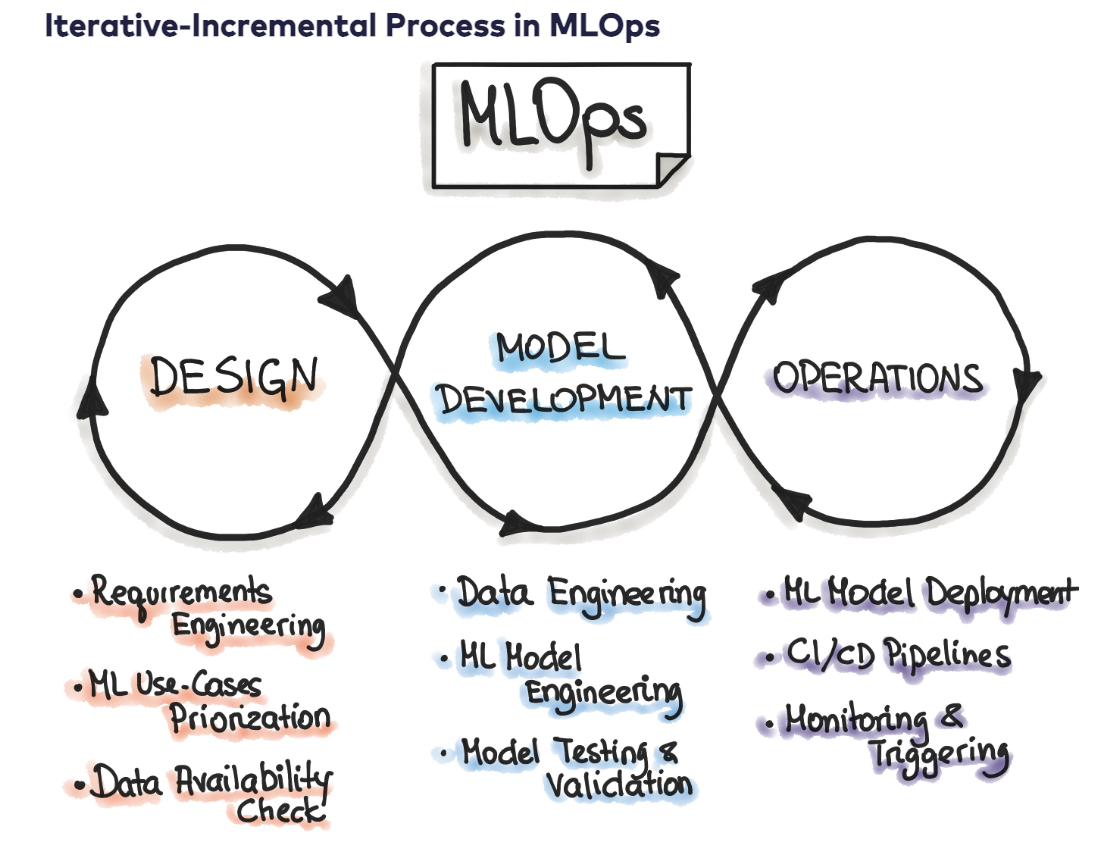
\includegraphics[width=\textwidth]{Images/Iterative MLOps.png}
	\caption{The complete MLOps process includes three broad phases of ``Designing the ML-powered application'', ``ML Experimentation and Development'',  and ``ML Operations''.}
	\label{fig:1}
\end{figure}
\FloatBarrier

MLOps leverages various tools to simplify the machine learning lifecycle.
\begin{itemize}[label={--}]
\item \textbf{Machine learning frameworks} like Kubernetes, TensorFlow and PyTorch for model development and training.
\item \textbf{Version control systems} like Git for code and model version tracking.
\item \textbf{CI/CD tools} such as Jenkins or GitLab CI/CD for automating model building, testing and deployment.
\item \textbf{MLOps platforms} like Kubeflow and MLflow manages model lifecycles, deployment and monitoring.
\item \textbf{Cloud computing platforms} like AWS, Azure and IBM Cloud provide scalable infrastructure for running and managing ML workloads.
\end{itemize}


\section{Environment Preparation}
\subsection{Configuring Environment with GitHub Codespaces}
To configure the environment using GitHub codespaces, first create a repository on GitHub, give the repository a name, add a ``README'' file and a \texttt{.gitignore} template, choose a license and create the repo. In the repo main page, click on \texttt{Create codespace on main} as shown in \textbf{Fig. \ref{fig:2}}.
\begin{figure}[h]
	\centering
	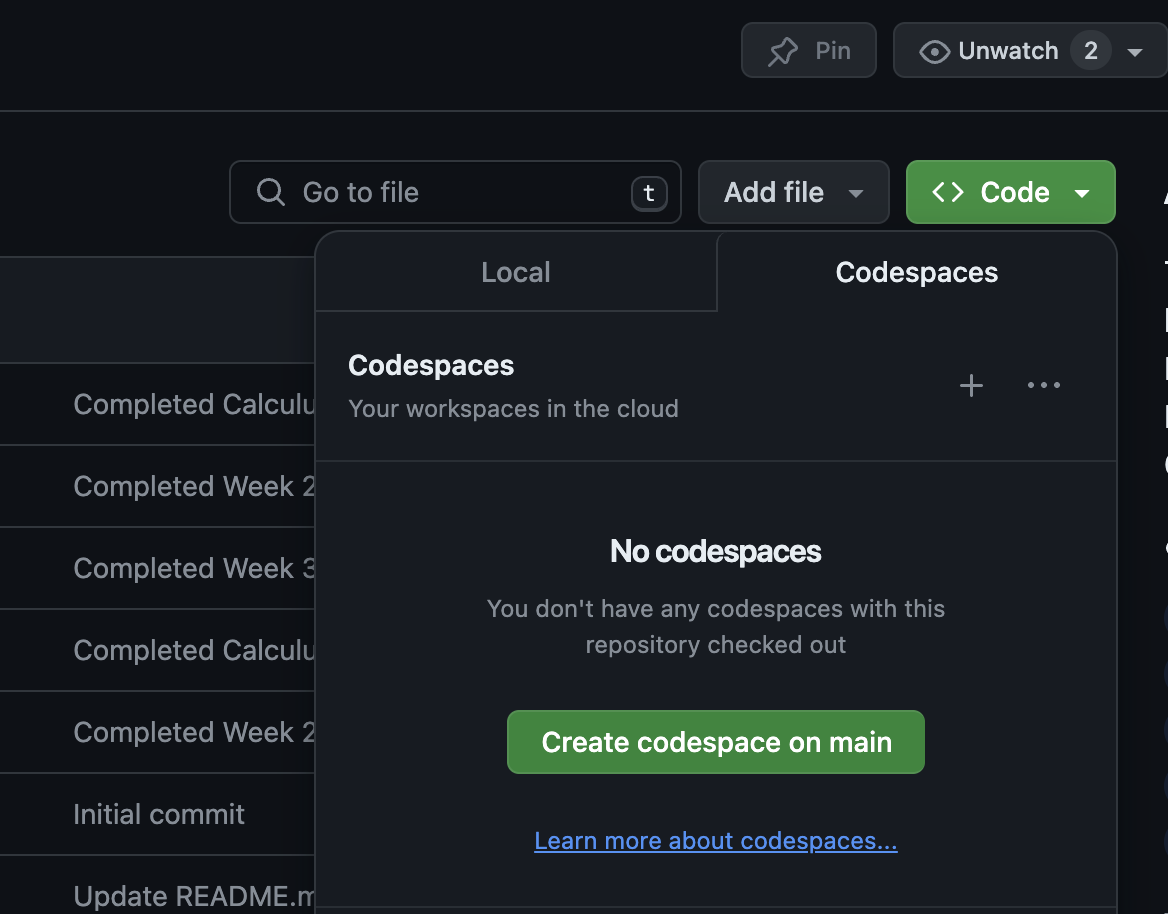
\includegraphics[width=0.5\textwidth]{Images/Codespaces.png}
	\caption{GitHub Codespaces setup}
	\label{fig:2}
\end{figure}
\FloatBarrier

A connection to Visual Studio Code can be made through Codespaces.  Start a new terminal, change directory to the workspaces and download and install Anaconda distribution of python in it using the step below.
 \begin{itemize}
\item \textbf{Step 1}: Download and install the Anaconda distribution of Python 
\begin{lstlisting}[language=python, numbers=none]
wget https://repo.anaconda.com/archive/Anaconda3-2022.05-Linux-x86_64.sh
\end{lstlisting}
\item \textbf{Step 2}: Run this command: 
\begin{lstlisting}[language=python, numbers=none]
bash Anaconda3-2022.05-Linux-x86_64.sh
\end{lstlisting}

After installing Anaconda, initialize it. In a new terminal, confirm that Anaconda is running in the workspaces
\begin{lstlisting}[language=python, numbers=none]
(base) @your_username -> /workspaces/mlops-zoomcamp-2024 (main) $ which python
/home/codespace/anaconda3/bin/python
\end{lstlisting}
\item \textbf{Step 3}: Make sure to install \texttt{pyarrow} in order to download parquet file
\begin{lstlisting}[language=python, numbers=none]
!pip install pyarrow
\end{lstlisting}
\item \textbf{Step 4}: Run jupyter notebook
\begin{lstlisting}[language=python, numbers=none]
jupyter notebook
\end{lstlisting}
\end{itemize}

\subsection{Configuring Environment with Amazon Web Service (AWS)}
To install using AWS,  create an account in AWS, go to EC2 and create an instance. Select the OS to use e.g. Ubuntu with 64-bit(x86) architecture. Select the instance type that will be sufficient for your project. Configure the cloud resources and launch. \\
Recommended development environment: Linux

 \begin{itemize}
\item \textbf{Step 1}: Download and install the Anaconda distribution of Python 
\begin{lstlisting}[language=python, numbers=none]
wget https://repo.anaconda.com/archive/Anaconda3-2022.05-Linux-x86_64.sh
bash Anaconda3-2022.05-Linux-x86_64.sh
\end{lstlisting}
\item \textbf{Step 2}: Update existing packages
\begin{lstlisting}[language=python, numbers=none]
sudo apt update
\end{lstlisting}
\item \textbf{Step 3}: Install Docker
\begin{lstlisting}[language=python, numbers=none]
sudo apt install docker.io
\end{lstlisting}
To run docker without sudo:
\begin{lstlisting}[language=python, numbers=none]
sudo groupadd docker
sudo usermod -aG docker \$USER
\end{lstlisting}
\item \textbf{Step 4}: Install Docker Compose \\
Install docker-compose in a separate directory
\begin{lstlisting}[language=python, numbers=none]
mkdir soft
cd soft
\end{lstlisting}
To get the latest release of Docker Compose, go to https://github.com/docker/compose and download the release for your OS.
\begin{lstlisting}[language=python, numbers=none]
wget https://github.com/docker/compose/releases/download/v2.5.0/docker-compose-linux-x86_64 -O docker-compose
\end{lstlisting}
Make it executable
\begin{lstlisting}[language=python, numbers=none]
chmod +x docker-compose
\end{lstlisting}
Add the soft directory to PATH. Open the .bashrc file with nano:
\begin{lstlisting}[language=python, numbers=none]
nano ~/.bashrc
\end{lstlisting}
In .bashrc, add the following line:
\begin{lstlisting}[language=python, numbers=none]
export PATH="${HOME}/soft:${PATH}"
\end{lstlisting}
Save it and run the following to make sure the changes are applied:
\begin{lstlisting}[language=python, numbers=none]
source ~/.bashrc
\end{lstlisting}
\item \textbf{Step 5}: Run Docker
\begin{lstlisting}[language=python, numbers=none]
docker run hello-world
\end{lstlisting}
\end{itemize}

\section{Model Development}
\subsection{Taxi trip prediction with machine learning}
    \begin{example}[frametitle=\extitle{TLC Trip Prediction}]
      In this section, we use machine learning to predict the trip duration for trips in New York. The data used were collected from the \href{https://www.nyc.gov/site/tlc/about/tlc-trip-record-data.page}{NYC Taxi and Limousine Commission (TLC)}. This dataset contains yellow and green taxi trip records include fields capturing pick-up and drop-off dates/times, pick-up and drop-off locations, trip distances, itemized fares, rate types, payment types, and driver-reported passenger counts. The data is stored in the PARQUET format.  We built a simple linear regression model and save the model as a pickle file for subsequent use later one.  See the \href{https://github.com/chuksoo/mlops-zoomcamp-2024/blob/main/01%20-%20Intro/duration-prediction.ipynb}{duration prediction notebook}.
    \end{example}

We can download parquet file using:
\begin{lstlisting}[language=python, numbers=none]
# download parquet data
!wget https://d37ci6vzurychx.cloudfront.net/trip-data/green_tripdata_2021-01.parquet
\end{lstlisting}

\section{MLOps Maturity Model}
The MLOps maturity model helps clarify the Development Operations (DevOps) principles and practices necessary to run a successful MLOps environment.  The maturity is the extent to which MLOps is implemented in a team. The MLOps maturity model encompasses five levels of technical capability.

% Please add the following required packages to your document preamble:
\begin{table}[H]
\resizebox{\columnwidth}{!}{%
\begin{tabular}{cp{2.5cm}p{7.0cm}p{7.0cm}}
\hline
Level & Description                     & Highlights                                                                                                                                                                                                                                         & Technology                                                                                                                                                                                   \\ \hline \hline
0     & No MLOps & \begin{itemize}[noitemsep, topsep=0pt]
    \item Hard to manage lifecycle
    \item Disparate teams
    \item Systems as ``black boxes''
\end{itemize}                 & \begin{itemize}[noitemsep, topsep=0pt]
    \item Manual builds/deployments
    \item Manual testing
    \item No centralized tracking
\end{itemize} \\ \hline
1     & DevOps but no MLOps            & \begin{itemize}[noitemsep, topsep=0pt]
   \item Less painful releases
    \item Limited feedback
    \item Hard to reproduce results
\end{itemize}              & \begin{itemize}[noitemsep, topsep=0pt]
    \item Automated builds
    \item Automated tests for application code
\end{itemize} \\ \hline
2     & Automated Training              & \begin{itemize}[noitemsep, topsep=0pt]
   \item Managed, traceable training
    \item Easy to reproduce model
    \item Low friction releases
\end{itemize}                      & \begin{itemize}[noitemsep, topsep=0pt]
    \item Automated model training
    \item Centralized tracking of model training performance
    \item Model management
\end{itemize} \\ \hline
3     & Automated Deployment     & \begin{itemize}[noitemsep, topsep=0pt]
    \item Releases are low friction and automatic
    \item Full traceability from deployment back to original data
    \item Entire environment managed: train > test > production
\end{itemize}                            & \begin{itemize}[noitemsep, topsep=0pt]
   \item Integrated A/B testing
    \item Automated tests for all code
    \item Centralized tracking
\end{itemize} \\ \hline
4     & Full MLOps Automated Operations & \begin{itemize}[noitemsep, topsep=0pt]
    \item Fully automated, monitored
    \item Systems provide improvement information
    \item Zero-downtime
\end{itemize} & \begin{itemize}[noitemsep, topsep=0pt]
    \item Automated training/testing
    \item Centralized metrics
\end{itemize}                                                              \\ \hline \hline
\end{tabular}%
}
\caption{Machine Learning operations maturity model (culled from \href{https://learn.microsoft.com/en-us/azure/architecture/ai-ml/guide/mlops-maturity-model}{Microsoft Blog}}
\label{tab:my-table}
\end{table}

%--------------- Chapter 2: Experiment Tracking and Model Management -----------%
\chapter{Experiment Tracking and Model Management} \label{ch:2}

\inspiration{MLOps is critical for the success of AI projects because it allows teams to iterate quickly and deploy machine learning models reliably and at scale.}{Andrew Ng}{}

\section{Introduction to Experiment Tracking}

 \begin{funfact}[frametitle=\facttitlep{Fun Fact}{MLflow}]
MLflow is an open-source platform that helps manage the end-to-end machine learning lifecycle. It provides a set of tools to streamline and automate various stages of the machine learning process, from experimentation to deployment. 
\end{funfact}

Machine Learning experiment is the process of building an ML model. Experiment run represents each trial in an ML experiment. A run artifact is any file associated with an ML run. The experiment metadata is all the information related to the experiment. \emph{Experiment tracking} is the process of keeping track of all the \textbf{relevant information} from an \textbf{ML experiment}, which includes:
\begin{itemize}[noitemsep, topsep=0pt]
	\item Source code
	\item Environment
	\item Data
	\item Models
	\item Hyperparameters
	\item Metrics
\end{itemize}

    \begin{mathaside}[frametitle=\mathtitle{Why is Experiment Tracking \color{firebrick}{so important}}]
      Experiment tracking is important because of \textbf{Reproducibility}, \textbf{Organization}, and \textbf{Optimization}
    \end{mathaside}

Experiment tracking is done using MLflow. MLflow is ``an open source platform for the machine learning lifecycle''. In practice, it's just a Python package that can be installed with pip, and it contains four main modules:
\begin{itemize}[noitemsep, topsep=0pt]
	\item Tracking
	\item Models
	\item Model Registry
	\item Projects
\end{itemize}

The MLflow Tracking module allows you to organize your experiments into runs, and to keep track of:
\begin{itemize}[noitemsep, topsep=0pt]
	\item Parameters
	\item Metrics
	\item Metadata
	\item Artifacts
	\item Models
\end{itemize}

Along with this information, MLflow automatically logs extra information about the run:
\begin{itemize}[noitemsep, topsep=0pt]
	\item Source code i.e., the name of the file that was used to run the experiment
	\item Version of the code (git commit)
	\item Start and end time
	\item Author
\end{itemize}

\subsection{How MLflow Helps Manage Machine Learning Experiments}
Here are some key ways in which MLflow can help with machine learning experiments:
\subsubsection{Experiment Tracking}
MLflow Tracking allows you to log and query experiments using APIs or a web-based interface. Key features include:

\begin{itemize}
    \item \textbf{Log Parameters and Metrics:} Easily log hyperparameters, metrics, and artifacts (such as model files) for each run.
    \item \textbf{Organize and Compare Runs:} Organize runs by experiments and compare results visually.
    \item \textbf{Search and Query:} Search and filter experiments using a web UI or API, allowing you to quickly find runs with specific attributes.
\end{itemize}

\subsubsection{Reproducibility}
MLflow promotes reproducibility of experiments by providing:

\begin{itemize}
    \item \textbf{Code Versioning:} Integrates with version control systems (like Git) to log the version of the code that produced a particular run.
    \item \textbf{Environment Management:} Capture and reproduce the software environment using Conda environments or Docker images.
    \item \textbf{Artifacts:} Store and retrieve artifacts such as datasets, models, and images, ensuring all elements of an experiment are preserved.
\end{itemize}

\subsubsection{Model Management}
MLflow Models facilitate model packaging, sharing, and deployment:

\begin{itemize}
    \item \textbf{Standardized Format:} Save models in a standardized format that includes the model itself along with its dependencies and environment.
    \item \textbf{Multi-Platform Support:} Export models to various formats (e.g., TensorFlow, PyTorch, scikit-learn) and deploy them to different environments (e.g., cloud services, Docker).
    \item \textbf{Model Registry:} Register and version models, track model lineage, and transition models through stages (e.g., ``staging'', ``production'').
\end{itemize}

\subsubsection{Deployment}
MLflow provides tools for deploying models to various platforms:

\begin{itemize}
    \item \textbf{Built-in Deployment Options:} Deploy models to cloud platforms like AWS SageMaker, Azure ML, and Google Cloud ML Engine.
    \item \textbf{Custom Deployments:} Create custom deployment logic using the MLflow REST API or the command-line interface (CLI).
    \item \textbf{Batch and Real-Time Serving:} Support for both batch and real-time serving of models, enabling various deployment scenarios.
\end{itemize}

\subsubsection{Collaboration}
MLflow facilitates collaboration among team members by providing:

\begin{itemize}
    \item \textbf{Centralized Tracking Server:} A centralized tracking server where team members can log and view experiment runs.
    \item \textbf{Sharing and Collaboration:} Share results, models, and insights easily within the team, fostering better collaboration and knowledge sharing.
    \item \textbf{Integration with CI/CD:} Integrate MLflow with continuous integration and continuous deployment (CI/CD) pipelines for automated testing and deployment of models.
\end{itemize}

\subsubsection{Scalability}
MLflow is designed to scale with your needs:

\begin{itemize}
    \item \textbf{Distributed Tracking:} Support for tracking experiments across distributed environments, making it suitable for large-scale machine learning projects.
    \item \textbf{Flexible Storage Options:} Use various backend storage systems for logging data, including file systems, databases, and cloud storage.
\end{itemize}

By integrating MLflow into your machine learning workflow, you can enhance the management, reproducibility, and deployment of your experiments. It provides a comprehensive set of tools that streamline the entire lifecycle of machine learning models, making it easier to track, reproduce, and deploy models at scale.


\section{Experiment tracking with MLflow}
To start experiment tracking, we need to create a conda environment for tracking experiment and activate it.
\begin{lstlisting}[language=python, numbers=none]
conda create -n exp-tracking-env python=3.9
conda activate exp-tracking-env
\end{lstlisting}

Once the environment is activated, install the ``requirements.txt'' file using:
\begin{lstlisting}[language=python, numbers=none]
pip install -r requirements.txt
\end{lstlisting}

Check the installed packages using:
\begin{lstlisting}[language=python, numbers=none]
pip list
\end{lstlisting}

To launch mlflow, and store all the artifacts in an sqlite database, we run:
\begin{lstlisting}[language=python, numbers=none]
mlflow ui --backend-store-uri sqlite:///mlflow.db --port 5001
\end{lstlisting}

If you encounter error when launching mlflow, use:
\begin{lstlisting}[language=python, numbers=none]
ps -A | grep gunicorn
\end{lstlisting} to view the processes using the port and kill them with:
\begin{lstlisting}[language=python, numbers=none]
kill <process number>
\end{lstlisting} before re-launching mlflow. 


To access mlflow ui, open \href{http://127.0.0.1:5001} in your browser. The mlflow interface is seen in \textbf{Fig. \ref{fig:3}}.
\begin{figure}[h]
	\centering
	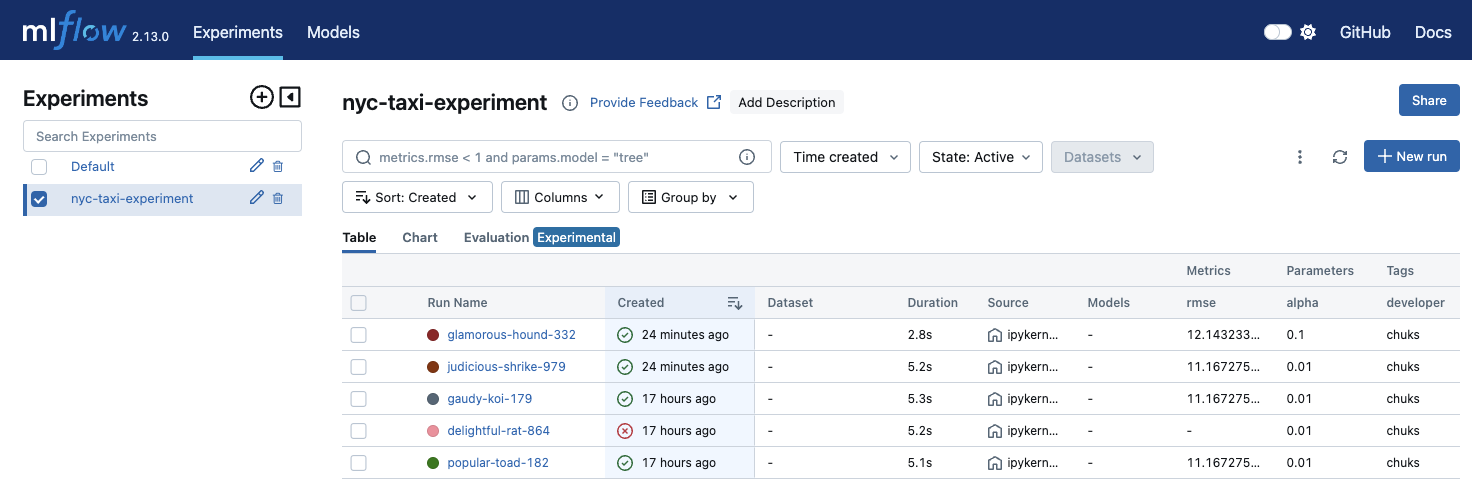
\includegraphics[width=\textwidth]{Images/mlflow-experiment-interface.png}
	\caption{MLflow Experiment Interface}
	\label{fig:3}
\end{figure}
\FloatBarrier

The updated notebook with experiment tracking using MLflow and logged predictions in MLflow UI is shown in this \href{https://github.com/chuksoo/mlops-zoomcamp-2024/blob/main/02%20-%20Experiment%20Tracking/duration-prediction.ipynb}{notebook for experiment tracking with mlflow}.

\section{Machine Learning Lifecycle}
 \begin{funfact}[frametitle=\facttitlep{Fun Fact}{MLOps cycle}]
The Machine Learning lifecycle refers to the multiple steps that are needed to build and maintain a machine learning model.
\end{funfact}

In Machine Learning Lifecycle,  we train some model, we tuned the hyperparameters, we evaluated the model and then logged some metrics, hyperparameters and other information needed to mlflow.  Once we finish with this experiment tracking stage, it means that we are happy with the model. Then we can start thinking of saving this model and have some kind of versioning. After that, we would like to deploy the model. We may realize that the model needs to be updated in order to scale. Finally, once we deploy the model, the prediction monitoring stage starts.

\begin{figure}[h]
	\centering
	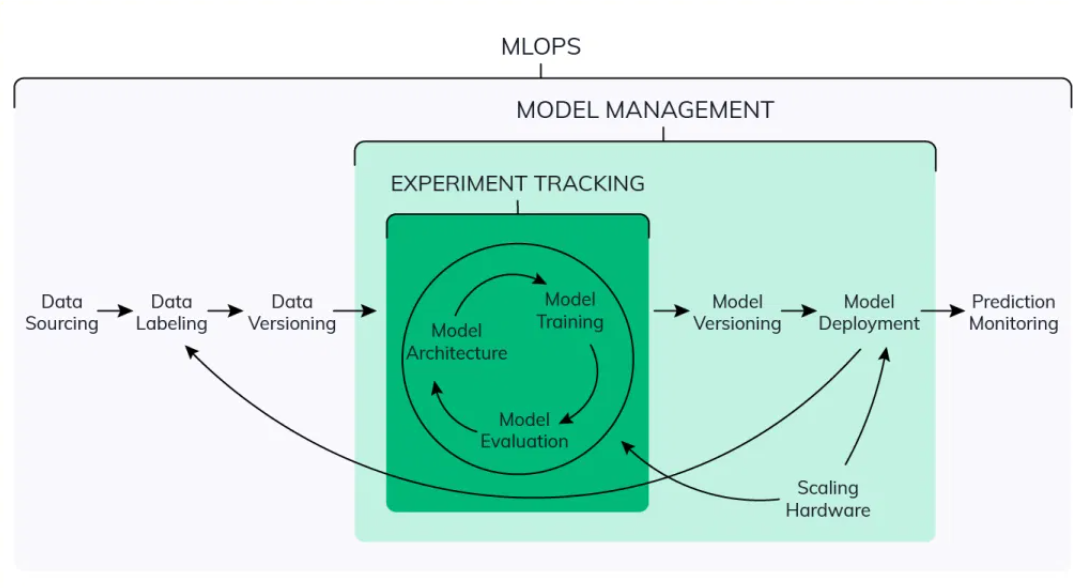
\includegraphics[width=\textwidth]{Images/neptune-mlops.png}
	\caption{MLOps cycle and machine learning experiment tracking}
	\label{fig:4}
\end{figure}
%\FloatBarrier

\subsection{Logging models in MLflow}
Two options :
\begin{itemize}[noitemsep, topsep=0pt]
\item Log model as an artifact
\begin{lstlisting}[language=python, numbers=none]
mlflow.log_artifact("<mymodel>", artifact_path="models/")
\end{lstlisting}
\item Log model using the method ``log\_model''
\begin{lstlisting}[language=python, numbers=none]
mlflow.<framework>.log_model(model, artifact_path="models/")
\end{lstlisting}
\end{itemize}

\subsection{Model Management}
Model management is a critical aspect of the machine learning lifecycle, encompassing the processes and tools used to effectively organize, version, and track machine learning models. Effective model management ensures that models can be deployed, monitored, and updated seamlessly, maintaining their performance and relevance over time. The main components of model management:

\subsubsection*{1. Versioning}
\begin{itemize}[noitemsep, topsep=0pt]
    \item \textbf{Importance:} Versioning allows data scientists to keep track of different iterations of a model, ensuring that they can reproduce results and compare performance across versions.
    \item \textbf{Tools:} Tools like MLflow, DVC, and Git provide functionalities to version models, track changes, and manage model metadata.
\end{itemize}

\subsubsection*{2. Deployment}
\begin{itemize}[noitemsep, topsep=0pt]
    \item \textbf{Purpose:} Deployment involves taking a trained model and making it available for inference in a production environment.
    \item \textbf{Methods:} Models can be deployed as a python function, in a docker container, as an APIs, embedded in applications, as a batch job in Apache Spark or integrated into data pipelines. Platforms like Kubernetes, AWS SageMaker, and Azure ML facilitate seamless deployment.
\end{itemize}

\subsubsection*{3. Monitoring}
\begin{itemize}[noitemsep, topsep=0pt]
    \item \textbf{Need:} Continuous monitoring of models in production is essential to ensure they perform as expected and to detect any performance degradation or data drift.
    \item \textbf{Metrics:} Key metrics to monitor include accuracy, latency, throughput, and error rates. Tools like Prometheus, Grafana, and custom logging solutions can be used for monitoring.
\end{itemize}

\subsubsection*{4. Retraining}
\begin{itemize}[noitemsep, topsep=0pt]
    \item \textbf{Process:} As new data becomes available, models may need to be retrained to maintain their performance.
    \item \textbf{Automation:} Automated retraining pipelines can be set up to periodically retrain models, incorporating the latest data and ensuring that the model remains up-to-date.
\end{itemize}

\subsubsection*{5. Governance and Compliance}
\begin{itemize}[noitemsep, topsep=0pt]
    \item \textbf{Compliance:} Ensuring that models comply with regulatory standards and organizational policies is crucial, especially in industries like finance and healthcare.
    \item \textbf{Documentation:} Proper documentation and audit trails are necessary for compliance and to provide transparency into how models are developed and used.
\end{itemize}

\subsubsection*{6. Collaboration}
\begin{itemize}[noitemsep, topsep=0pt]
    \item \textbf{Teamwork:} Effective model management facilitates collaboration among data scientists, engineers, and business stakeholders.
    \item \textbf{Tools:} Collaborative tools like Jupyter Notebooks, GitHub, and MLflow allow teams to share code, experiments, and insights.
\end{itemize}

\subsection*{Benefits of Effective Model Management}
\begin{itemize}[noitemsep, topsep=0pt]
    \item \textbf{Reproducibility:} Ensures that models can be consistently reproduced, which is crucial for validation and debugging.
    \item \textbf{Scalability:} Facilitates the scaling of machine learning efforts across an organization.
    \item \textbf{Efficiency:} Streamlines the deployment and monitoring processes, reducing time to market for new models.
    \item \textbf{Compliance:} Helps maintain compliance with legal and regulatory requirements.
\end{itemize}

In summary, model management is essential for maintaining the lifecycle of machine learning models, from development through deployment and monitoring, ensuring they continue to deliver value and perform optimally in production environments.

\subsection{Model Registry in Machine Learning}

    \begin{mathaside}[frametitle=\mathtitle{Why Model \color{firebrick}{registry}}]
            Model registry is an essential tool for managing the lifecycle of machine learning models, ensuring that they are well-organized, reproducible, and efficiently deployable, while enhancing collaboration and compliance within an organization.
    \end{mathaside}

A model registry is a centralized repository that stores and manages machine learning models. It plays a crucial role in the machine learning lifecycle by providing a systematic way to organize, version, and track models. The key components and benefits of a model registry:

\textbf{1. Versioning}
\begin{itemize}[noitemsep, topsep=0pt]
    \item \textbf{Purpose:} Keeps track of different iterations and versions of a model.
    \item \textbf{Functionality:} Allows comparison of model performance over time and ensures reproducibility.
\end{itemize}

\textbf{2. Metadata Management}
\begin{itemize}[noitemsep, topsep=0pt]
    \item \textbf{Purpose:} Stores important information about models, such as hyperparameters, training data, and evaluation metrics.
    \item \textbf{Functionality:} Facilitates model auditability and governance.
\end{itemize}

\textbf{3. Lifecycle Management}
\begin{itemize}[noitemsep, topsep=0pt]
    \item \textbf{Purpose:} Manages the lifecycle of models from development to deployment and monitoring.
    \item \textbf{Functionality:} Ensures smooth transitions between different stages of the model lifecycle.
\end{itemize}

\textbf{4. Access Control}
\begin{itemize}[noitemsep, topsep=0pt]
    \item \textbf{Purpose:} Defines who can access and modify models in the registry.
    \item \textbf{Functionality:} Enhances security and ensures that only authorized users can make changes.
\end{itemize}

\textbf{5. Deployment Integration}
\begin{itemize}[noitemsep, topsep=0pt]
    \item \textbf{Purpose:} Facilitates the deployment of models to production environments.
    \item \textbf{Functionality:} Provides integration with deployment tools and platforms for seamless model serving.
\end{itemize}

As we continue to generate more models, we need a model registry consisting of a tracking server to keep track of the models. Once you've decided that some of the model are ready for production, you then register the model into the mlflow model registry. Within the model registry, we have a staging , production and archive area for the models. In the model registry, all the models that are ready for production are stored here. 

\begin{figure}[h]
	\centering
	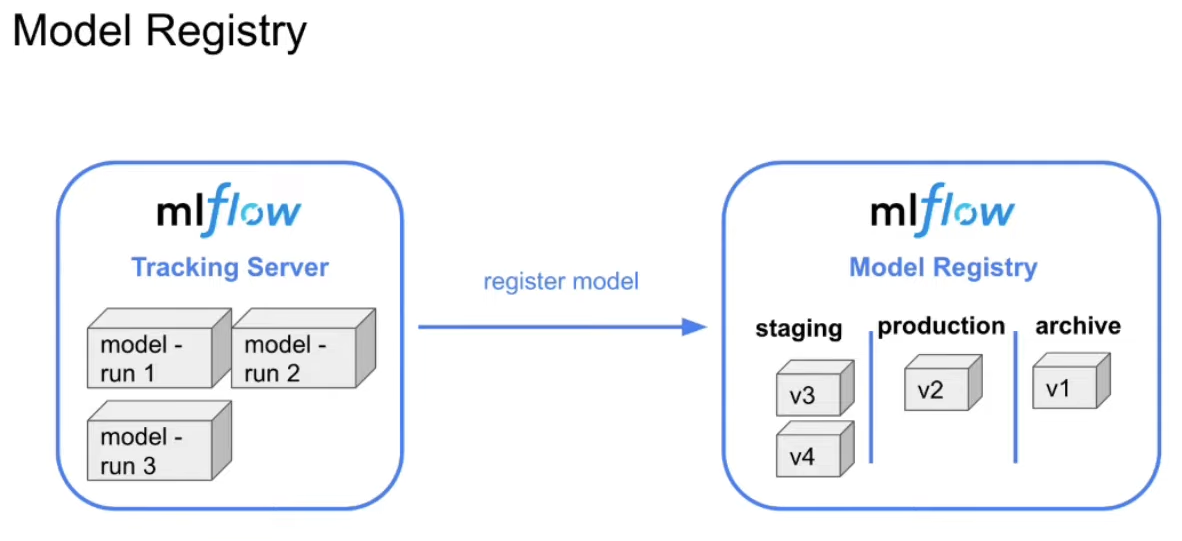
\includegraphics[width=\textwidth]{Images/model registry.png}
	\caption{Model Registry}
	\label{fig:5}
\end{figure}
\FloatBarrier

The MLOps Engineer can look at the models in the registry, inspect their hyperparameters, the size of the model and so on. He can then decide to move the models between the different stages. The model that is ready for production can be assigned to ``staging'', the current model that is used in production can be assigned to the ``production'' stage, and some of the models can be archived in the ``archived'' stage. The archived models can be retrieved from the archived stage and move them back to production if we want to roll back some deployments. The model registry is not deploying any model, it just lists the models that are production ready and the stages are just labels assigned to the model. The model registry will need to be complemented with some CI/CD code in order to do the actual deployment of the models. 

    \begin{mathaside}[frametitle=\mathtitle{Using \color{firebrick}{MLflowClient}}]
           \texttt{mlflow.client} is a module in MLflow that provides a way to interact programmatically with an MLflow tracking server. The primary class in this module is MlflowClient, which provides a comprehensive API for managing experiments, managing runs, models, logging artifacts, and interacting with model registry. 
    \end{mathaside}

\subsection{Interacting Programmatically with MLflowClient}
The \texttt{mlflow.client} module is useful for advanced use cases where you need programmatic control over MLflow entities, especially in production environments where automated workflows and integrations are required.

Here's a basic example demonstrating how to use \texttt{MlflowClient}:

\begin{lstlisting}[language=Python, caption=Example Usage of \texttt{MlflowClient}, label=code:example]
import mlflow
from mlflow.tracking import MlflowClient

# Initialize the client
client = MlflowClient()

# Create an experiment
experiment_id = client.create_experiment("My New Experiment")

# Start a new run in the experiment
run = client.create_run(experiment_id)
run_id = run.info.run_id

# Log parameters, metrics, and tags
client.log_param(run_id, "param1", 5)
client.log_metric(run_id, "metric1", 0.89)
client.set_tag(run_id, "tag1", "value1")

# Log an artifact (a file)
with open("output.txt", "w") as f:
    f.write("Hello, world!")
client.log_artifact(run_id, "output.txt")

# End the run
client.set_terminated(run_id)

# Get information about the run
run_info = client.get_run(run_id)
print(run_info)
\end{lstlisting}

\subsubsection{Key Methods of \texttt{MlflowClient}}

\subsubsection*{1. Experiment Management}
\begin{itemize}
    \item \texttt{create\_experiment(name, artifact\_location=None, tags=None)}: Creates a new experiment.
    \item \texttt{get\_experiment(experiment\_id)}: Retrieves an experiment by ID.
    \item \texttt{delete\_experiment(experiment\_id)}: Deletes an experiment.
\end{itemize}

\subsubsection*{2. Run Management}
\begin{itemize}
    \item \texttt{create\_run(experiment\_id, start\_time=None, tags=None)}: Starts a new run.
    \item \texttt{log\_param(run\_id, key, value)}: Logs a parameter.
    \item \texttt{log\_metric(run\_id, key, value, timestamp=None, step=None)}: Logs a metric.
    \item \texttt{set\_tag(run\_id, key, value)}: Sets a tag.
    \item \texttt{log\_artifact(run\_id, local\_path, artifact\_path=None)}: Logs an artifact.
\end{itemize}

\subsubsection*{3. Model Registry Management}
\begin{itemize}
    \item \texttt{create\_registered\_model(name)}: Creates a new registered model.
    \item \texttt{create\_model\_version(name, source, run\_id, tags=None, run\_link=None, description=None)}: Creates a new model version.
    \item \texttt{transition\_model\_version\_stage(name, version, stage)}: Transitions a model version to a new stage.
\end{itemize}

\section{MLflow in Practice}
\subsection{Different scenarios for running MLflow}
Let's consider these three scenarios:
\begin{itemize}[noitemsep, topsep=0pt]
\item \textbf{\smtt{A single data scientist participating in an ML competition}}: In this scenario, having remote tracking server will be an overkill. Saving this information locally will be enough. Also, using model registry is useless since the data scientist is not deploying this model to production.
\item \textbf{\smtt{A cross-functional team with one data scientist working on an ML model}}:Here, sharing the experiment information is important. Also, using model registry will be a good idea but it can be run remotely or local host.
\item \textbf{\smtt{Multiple data scientists working on multiple ML models}}: Since multiple data scientist are working on multiple model, collaboration and sharing experiment information is very important. One data scientist can build the model, another data scientist can tune different hyperparameters to add to the model. They need a way to keep track of the models using a remote tracking server. Also, it is important to manage the lifecycle of the model since multiple people build and deploy the model hence model registry is important. 
\end{itemize}

\subsection{Things to Consider before Configuring MLflow}
There are different things to consider before configuring MLflow.
\begin{itemize}[noitemsep, topsep=0pt]
\item \textbf{Backend Store}: Where MLflow saves information about your experiement such as metadata, models etc
	\begin{itemize}[label={\ding{224}}]
		\item local filesystem
		\item SQLAlchemy compatible DB (e.g. SQLite)
	\end{itemize}
\item \textbf{Artifacts Store}: Decide where to store the artifact i.e., locally or remote
	\begin{itemize}[label={\ding{224}}]
		\item local filesystem
		\item remote (e.g.  s3 bucket)
	\end{itemize}
\item \textbf{Tracking Server}: Decide how to run tracking server
	\begin{itemize}[label={\ding{224}}]
		\item no tracking server
		\item localhost
		\item remote
	\end{itemize}
\end{itemize}




%
\begin{itemize}
  \item Like this one,
    \begin{notebox}
      which is wrapped in gray. I use it for notes.\ldots
    \end{notebox}

  \item Or this one,
    \begin{funfact}
      which is wrapped in red. I use it for fun facts or other asides\ldots
    \end{funfact}

  \item Or this one,
    \begin{mathaside}
      which is wrapped in blue and used for mathy stuff.
    \end{mathaside}

  \item Or this last one,
    \begin{example}
      which is wrapped in green. With a title, it's used for enumerated examples
      (see \smtt{\textbackslash extitle} and \smtt{\textbackslash excounter}).
      Observe:
    \end{example}

    \begin{example}[frametitle=\extitle{Test}]
      This is an example. What's the answer to $2+2$?
      \answer{Obviously 4, lol.}
    \end{example}

    \begin{example}[frametitle=\extitle{Test Again}]
      This one will increment the counter automatically, resetting for each
      chapter.
    \end{example}


  \item For red and blue boxes, there are custom commands for titles, too:
    \begin{mathaside}[frametitle=\mathtitle{One Title}]
      Like this
    \end{mathaside}
    \begin{mathaside}[frametitle=\mathtitlep{Two Titles}{A Subtitle}]
      Or this
    \end{mathaside}
\end{itemize}

\hr{5in}

These styles also automatically apply to theorems and claims.

\begin{theorem}[Pythagorean Theorem]
  \label{thm:pyth}
  For any right triangle with legs $a,b$ and hypotenuse $c$:
  %
  \begin{equation}
    \label{eq:pyth}
    a^2+b^2=c^2
  \end{equation}
\end{theorem}
\begin{proof}
  This is left as an exercise to the reader.
\end{proof}

\begin{claim}
  This is the greatest note template in the world.
\end{claim}

\hr{5in}

There are different ways to quote things, too, depending on how you want to
emphasize:

\begin{quoting}
  This is a simple, indented quote with small letters and italics usually
  suitable for in-text quotations when you just want a block.
\end{quoting}

Alternatively, you can use the \smtt{\textbackslash inspiration} command from
the chapter heading, which leverages the \smtt{thickleftborder} frame
internally, but adds a little more padding and styling (there's also just
\smtt{leftborder} for a thinner variant):

\begin{thickleftborder}
  Hello there!
\end{thickleftborder}



\section{On Cross-Referencing}
\marginnote{\footnotesize\softtext This is the standard way to include margin
notes. There are also commands to link to source papers directly (see
\smtt{\textbackslash lesson}).} You can reference most things---see
\autoref{thm:pyth} or \eqref{eq:pyth} or the \nameref{ch:1} chapter---directly
and easily as long as you give them labels. These are ``built-ins.'' However,
you can also create a \term{custom term} that will be included in the index,
then include references to it that link back to the original definition. Try
clicking: \refterm{custom term}. Building the index is on you, though. You can
also reference by using a different term for the text: \reftermx{custom
term}{like this}. Sometimes it doesn't fit the \termx{grammar}{grammatical
structure} of the sentence so you can define the term one way and visualize it
another way (this creates a \aterm{grammar} entry in the index). There's also
\prop{math terms} and a way to reference them: \refprop{math terms} (clickable),
but they do \textbf{not} show up in the index.



\section{On Math}
Most of the math stuff is just macros for specific things like the convolution
operator, $\conv$, probabilities, $\cprob{A}{B=C}$, or big-$O$ notation,
$\bigO{n^2\log{n}}$ but there's also a convenient way to include explanations on
the side of an equation:
%
\begin{align*}
  1 + 1 &\overset{?}{=} 2    \sideblock{2in}{first we do this} \\
      2 &\overset{?}{=} 2    \sideblock{2in}{then we do this} \\
      2 &= 2 \qed
\end{align*}

These are all in the \smtt{CustomCommands.sty} file.



\end{document}

